\chapter{Modelling the Whole Atrium}

In the previous chapter a modelling library suitable for simulation of single
cell, 1D and 2D cardiac tissue was developed.
This library was used to investigate aspects of atrial electrical activity.
These models provide valuable insight into the behaviours of cardiac tissue in health
and disease.
However, these simple models ignore the complex 3D structure of the atria.
This complexity can be seen internally, in that the atrium is comprised of several
distinctive tissue types with different cellular electrophysiological properties
and inter-cellular electrical coupling.
It can also be seen in the gross physical structure, the atrium has a complex
topology with both holes for the venous and arterial openings, as well as
openings for the valves.
The simpler, often idealized, models constructed in the previous chapter
ignore (and in many cases, are incapable of showing) many of these complexities.
To provide insight into the atrium function on the whole organ level one must
therefore simulate the atrium as an organ.
A 3D model of the atrium requires a representation of the atrial geometry to
provide the topology of the atrium.
To model complexities with sufficient accuracy models of the
electrophysiologically distinct tissue types are also required as are
descriptions of the complex conductivities.


\section{Anatomical Atrial Geometry}
\label{atrium:sec:geometry}

The anatomical atrial geometry used in the simulation studies presented here was based on
the visible human project female dataset.
The visible human dataset was created from a pair of cadavers, set into wax and
sliced into \mm{1}\ and \mm{0.33}\ for the male and female bodies, respectively.
The geometric model used here was extracted from the female dataset and so has a
spatial resolution of \mm{0.33}.
The extracted anatomical geometry is segmented into different tissue types,
with distinct classifications for left and right atrium, the pectinate muscles,
the crista terminalis, the Bachmann bundle and the sino-atrial node, as shown in
figure~\ref{atrium:geometry}.
The geometry has been used in numerous previous simulation studies.
It was discretised via a finite differences approach, which
allows the whole atrium to be embedded in a block of $298\times269\times235$
nodes.
This gives it a size of approximately 19 million nodes, although only
approximately 1.6 million of those nodes correspond to atrial cells.
The anatomical model also considers fibre orientation in the pectinate muscles,
crista terminalis and Bachmann bundle, which always run parallel to the local
axis of the tissue bundle, as determined by principle component
analysis~\cite{Seemann2006}.
Representations of the fibre structure are shown in figure~\ref{atrium:fibres}.

\begin{figure}
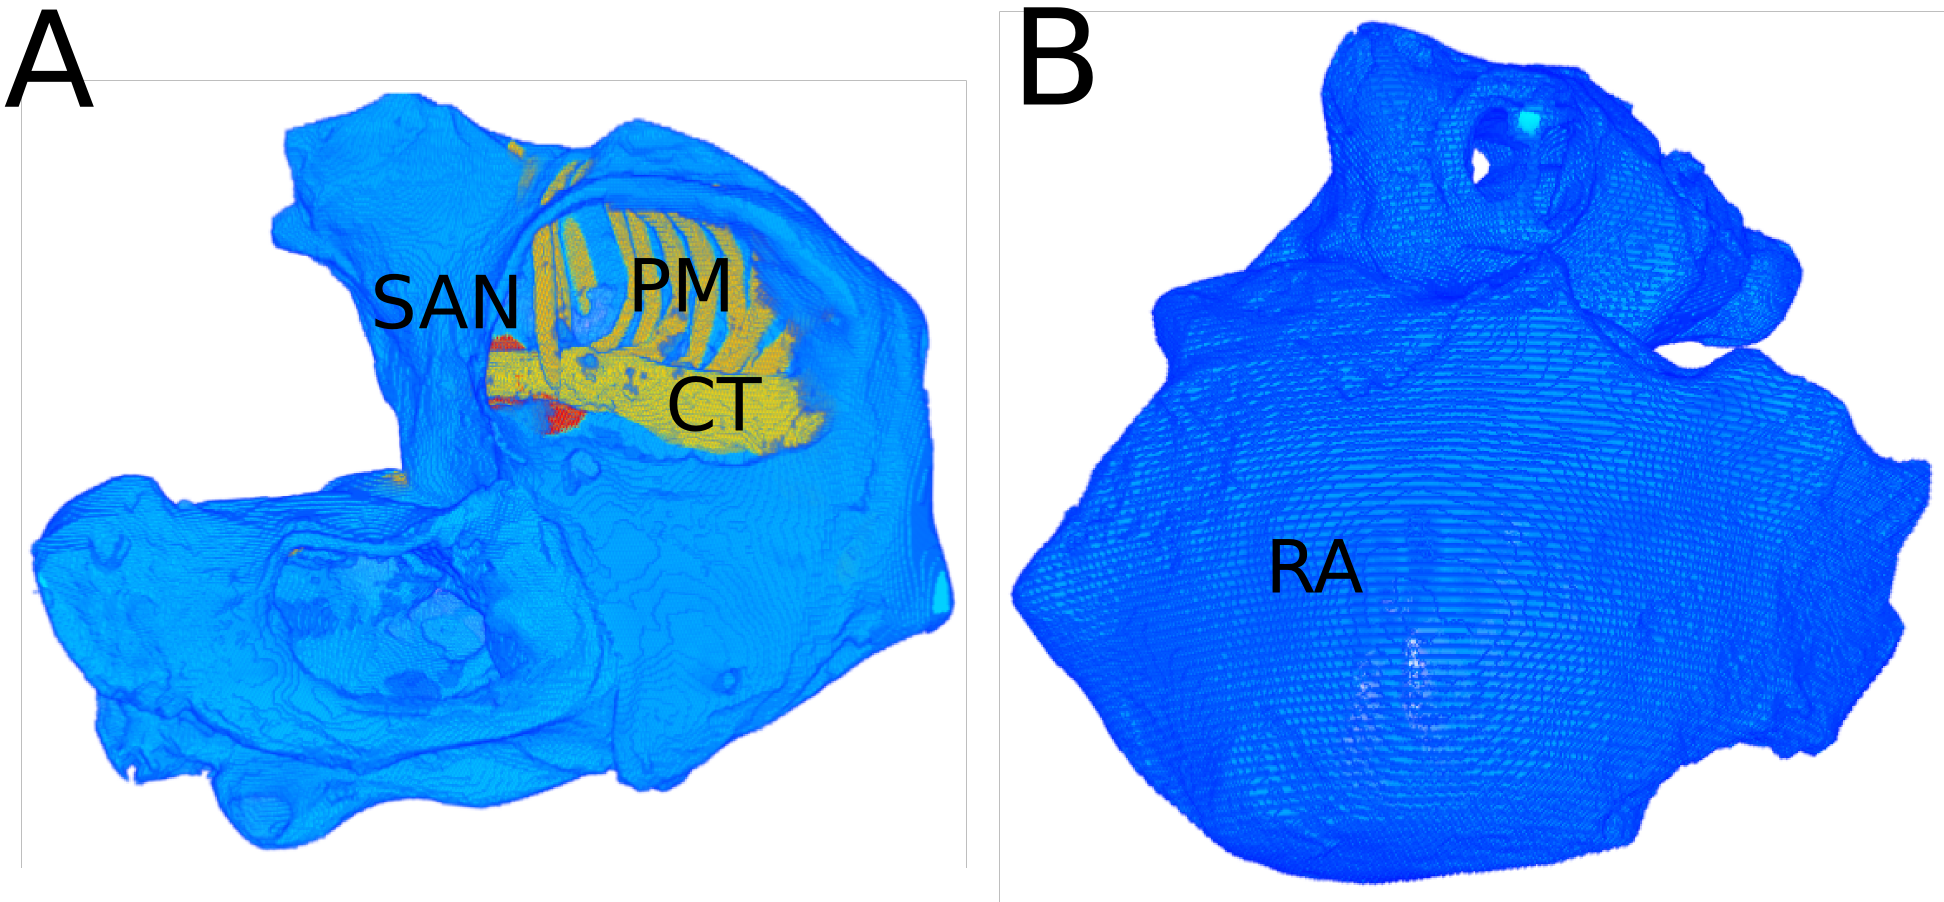
\includegraphics{figures/atrium/structure/atrial_geometry}
\caption[Atrial Geometry]{
\label{atrium:geometry}
(a)
View up into the right (RA) and left (LA) atria, showing the pectinate muscles
(PM, orange), crista terminalis (CT, yellow) and sino-atrial node (SAN, red).
The atrial muscle is shown in blue.
Also labelled are the right (RAA) and left (LAA) appendages.
(b)
A view of the atrial geometry looking down onto the wall of the right
atrium.  Visible at the top of the panel is the opening for one of the pulmonary
veins (PV).
}
\end{figure}

\begin{figure}
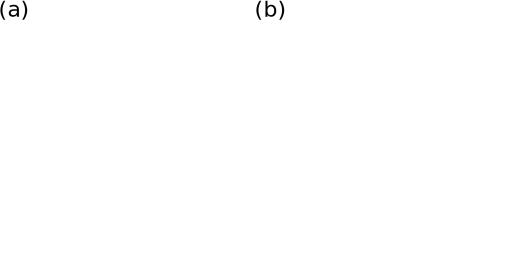
\includegraphics{figures/atrium/structure/fibres}
\caption[Atrial Fibre Structure]{
\label{atrium:fibres}
Representation of the fibre structure of the atrial geometry from a frontal
view (a) and a view up into the atria from the ventricles (b).
The arrows in red are aligned along the unit vectors of the fibre orientation.
The crista terminalis and the pectinate muscles are very easy to see with their
well defined fibre orientation.
}
\end{figure}

\section{Simulation Methods}
\label{atrium:sec:model}

\subsection{Atrial Model}

The electrical activity at each of the nodes was described by the equations of
the Courtemanche--Ramirez--Nattel (CRN) of the human atrial
myocyte~\cite{CRN98}.  This model, as previously described, is a second
generation model. It has 21 state variables, representing ionic gating activations
and inactivations and intracellular concentrations of ionic species.  In the
model, the total current, \ii{ion} is made up of the contributions of numerous
ion channels and exchangers.
\begin{equation}
\label{atrium:crn}
\ii{ion} = \ii{Na} + \ii{K1} + \ii{to} + \ii{Kur} + \ii{Ks} + \ii{Kr} +
\ii{Ca,L} + \ii{p,Ca} + \ii{NaK} + \ii{NaCa} + \ii{b,Na} + \ii{b,Ca}
\end{equation}
where \ii{Na}, \ii{K1}, \ii{to}, \ii{Kur}, \ii{Ks}, \ii{Kr}, \ii{Ca,L},
\ii{p,Ca}, \ii{b,Na} and \ii{b,Ca}\ represent ionic currents and \ii{NaK}\ and
\ii{NaCa}\ are ion exchangers.  As a second generation model, the CRN model also
has a detailed calcium handling system which can influence the action potential
via its influence on the intracellular calcium concentration.

In some atrial simulations it was desirable to incorporate details of
electrophysiological heterogeneity to represent the regional difference in
electrical activity of atrial myocytes and the other cellular types present in
the geometry, such as the pectinate muscles and crista terminalis.
The parameters used for
heterogeneity were based on measurements taken by Feng et al.~\cite{Feng1998}
of the canine atrium.  These were converted to parameters for the CRN model by
Seemann et al.~\cite{Seemann2004} and have been used in several simulation
studies~\cite{Seemann2006,Stott2008}.  They are shown in
table~\ref{atrium:het_params}.

\begin{table}
\caption[Tissue Heterogeneity Parameters]{
\label{atrium:het_params}
Table showing the parameters altered to differentiate pectinate muscle (PM) and
crista terminalis (CT) cells, compared to the normal Courtemanche et al. (CRN)
parameters.
}
\begin{center}
\begin{tabular}{r c c c}
\toprule
 & CRN & PM & CT \\
\midrule
\g{to,max} & 0.1652 & 0.1652 & 0.2215 \\
\g{Ca,L,max} & 0.1238 & 0.1238 & 0.2067 \\
\g{Kr,max} & 0.0294 & 0.0294 & 0.0294 \\
\bottomrule
\end{tabular}
\end{center}
\end{table}

\subsection{Monodomain Equation}

To simulate the propagation of electrical activity over the finite difference
geometry previously described, the mono-domain equation is used to describe the
changes in $V$ in time, $t$, the trans-membrane voltage.
\begin{equation}
\label{atrium:monodomain}
\frac{\partial V}{\partial t} = \nabla\cdot D \nabla V - \frac{\ii{ion}}{C_{m}}
\end{equation}
where $D$ is a tensor representing the diffusivity of electrical potential, \ii{ion} is described by the
CRN model (\ref{atrium:crn}), $C_{m}$ is the membrane capacitance and all other
symbols have their usual meanings.  Equation (\ref{atrium:monodomain}) is
advanced in time via the forward Euler method with a timestep of \ms{0.02}.  For
simulations with isotropic conductivity between nodes a 7-node approximation of
the differential operator is used.  When anisotropy is present, a 19-node
approximation is used.

\subsection{Tissue Anisotropy}

The heart has a complex fibrous structure (Chapter 1), and this manifests
electrically as regions which have preferential conduction directions.
The preferential conduction directions show greatly increased conduction
velocities, sometimes by a factor of up to five~\cite{}.
The fibre structure and regions of preferential conduction are generally
considered much more important for the ventricles than for the atria.
The atria, or more specifically the right atrium, do possess several structures
with a definite direction of preferential conduction.
These are the crista terminalis, responsible for rapid conduction of the
depolarization wave to the atrio-ventricular node, the pectinate muscles and the
Bachmann bundle, the preferential pathway for conduction between the atria.
To determine the influence of anisotropic conduction on the propagation of the
electrical activity, we follow a method after Panfilov and
Keener~\cite{Panfilov1995}.
In this method there is a unit vector, $\mathbf{f}$, defined at every point in
the tissue which has significant fibre orientation.
This unit vector defines a set of co-ordinate axes, in which the conductivity
tensor is diagonal
\begin{equation}
\label{atrium:dtilde}
\mathbf{\tilde{D}} =
\begin{pmatrix}
D_{\parallel} & 0 & 0\\
0 & D_{\perp} & 0\\
0 & 0 & D_{\perp}
\end{pmatrix}
\end{equation}
where $D_{\parallel}$ is the diffusion constant for conduction parallel to the
preferential direction of conduction and $D_{\perp}$ is the diffusion constant
for conduction perpendicular to this direction.
In this formulation it is assumed that there is no `sheet' structure which gives
a higher conduction velocity in one direction perpendicular to the main fibre
axis.
The diffusion tensor $\mathbf{\tilde{D}}$\ will only be diagonal in the
Cartesian co-ordinate system of the heart if the direction of preferential
conduction is parallel to one of the axes.
Therefore, to find the conductivity tensor in the global co-ordinate system,
$\mathbf{D}$, we need to find two transformation matrices $\mathbf{A}$\ and
$\mathbf{A^{T}}$\ such that
\begin{equation}
\label{atrium:d}
\mathbf{D} = \mathbf{A} \mathbf{\tilde{D}} \mathbf{A^{T}}
\end{equation}
To find $\mathbf{A}$\ it is possible to write out the involved rotations
explicitly, however an alternative method~\cite{Fenton2005}\ uses the fact that
$\mathbf{f}$\ and the two vectors orthogonal to it, $\mathbf{g}$\ and
$\mathbf{h}$\ are eigenvectors of $\mathbf{D}$.
These have the eigenvalues of $D_{\parallel}$\ and $D_{\perp}$.
The matrix $\mathbf{A}$\ is therefore an orthogonal matrix of the form
$\mathbf{A} = \left(\mathbf{f},\mathbf{g},\mathbf{h}\right)$ and so, using
(\ref{atrium:d}) $\mathbf{D}$\ can be written as
\begin{equation}
\label{atrium:dfgh}
\mathbf{D} = D_{\parallel}\mathbf{f}\mathbf{f^{T}} +
D_{\perp}\left(\mathbf{g}\mathbf{g^{T}} + \mathbf{h}\mathbf{h^{T}}\right)
\end{equation}
Using the fact that $\mathbf{A}\mathbf{A^T} = \mathbf{I}$ it is possible to
write
\begin{equation}
\label{atrium:dwithf}
\mathbf{D} = D_{\perp}\mathbf{I} + \left(D_{\parallel}-D_{\perp}\right)\mathbf{f}\mathbf{f^{T}}
\end{equation}
where $\mathbf{I}$\ is the identity matrix, and all other symbols are as defined
previously.
The directions of preferential conduction for the atrial geometry used in the
study were described by a pair of angles $\theta$\ and $\phi$\ representing the
orientation of the unit vector $\mathbf{f}$\ at each point in spherical polar
co-ordinates.
In cells with no assigned preferential conduction direction, the components of
$\mathbf{f}$\ were set to zero, giving a diffusion tensor of
\begin{equation}
\label{atrium:dnofibre}
\mathbf{D} =
\begin{pmatrix}
D_{\perp} & 0 & 0\\
0 & D_{\perp} & 0\\
0 & 0 & D_{\perp}
\end{pmatrix}
\end{equation}
which is the diffusion tensor for isotropic conduction.

The fibre orientations for the anatomical geometry used in this study are
defined in two files.
These two files contain the theta and phi components of the fibre vectors
between $0$ and $\pi$, discretised in 255 steps.
The relationship between the angles theta and phi and the unit vector of fibre
direction, $\mathbf{f}$, are shown in
figure~\ref{fig:atrium:structure:unit_vector}.
\begin{figure}
\begin{center}
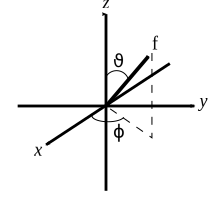
\includegraphics{figures/atrium/structure/unit_vector}
\end{center}
\caption[Relationship of $\theta$, $\phi$ and $\mathbf{f}$]{
\label{fig:atrium:structure:unit_vector}
The relationship of the angles $\theta$ and $\phi$ with the unit vector of fibre
orientation, $\mathbf{f}$.
The angle $\theta$ is the angle between the $z$ axis and $\mathbf{f}$.
The angle $\phi$ is the angle of rotation of $\mathbf{f}$ around the $z$ axis in
the $x\text{--}y$ plane.
}
\end{figure}
To convert theta and phi to the unit vector $\mathbf{f}$ we
use~\cite{Misner1973},
\begin{subequations}\label{eqn:atrium:structure:anglestof}
\begin{align}
f_x &= \cos\phi \sin\theta \label{eqn:atrium:structure:anglestofx}\\
f_y &= \sin\phi \sin\theta\label{eqn:atrium:structure:anglestofy}\\
f_z &= \cos\theta\label{eqn:atrium:structure:anglestofz}
\end{align}
\end{subequations}
where $\theta$ and $\phi$ are as indicated in
figure~\ref{fig:atrium:structure:unit_vector}\ and $f_x$, $f_y$, $f_z$ are the
$x$--, $y$--, $z$-- components of the vector $\mathbf{f}$.





\subsection{Computational Implementation}

The atrial geometry used in these studies is quite large, consisting of almost
19 million nodes.
As noted in \ref{atrium:sec:geometry}, only approximately 1.6 million of these
nodes correspond to active tissue--less than 10\% of the total.
The electrical activity at each node is represented by the CRN model and thus
requires 21 double precision numbers to be stored, representing the state
variables of the model.
The memory requirements of the model may be significantly reduced by storing
state variables, and where anisotropy is present the diffusion tensor, only for
the active nodes.
This reduces the memory requirements for storing the state variables from
approximately \unit{2.9}{GB}\ to \unit{256}{MB}.
A further simplification may be obtained by decomposing the geometry into a
linear array, containing the 6 or 18 neighbours of the active nodes to be used
in the diffusion tensor approximation.
The geometry and state information can therefore be represented by one linear
array of cellular states, one linear array used as a `map' and one
linear array representing the components of the Laplacian.
This linear data structure is very easy to parallelize on a shared memory
system.

The parallelization was accomplished through the use of the OpenMP shared
memory parallelism library~\cite{OpenMP}.
The system was then solved on 1 node of the Horace supercomputer on a total of 8
cores.
The linear array of active nodes was divided equally between the 8 cores, with
each core solving (\ref{atrium:crn}) for all nodes its assigned section of the
array.
A snapshot of the trans-membrane potentials at each of the active node sites was
output every \ms{1}\ of simulated time.
Simulation of \unit{1}{s}\ of atrial activity took 3.4 hours.
A parallel fraction of XXXX was attained, indicating that almost all of the
workload was effectively distributed over the 8 cores.

\section{Validation of the Model}

To verify the model, it was used to simulate a normal propagation, initiated
from the sino-atrial node.
The fully detailed model was used.
The Laplacian was precomputed to include all the information on tissue
anisotropy from the fibre orientation which accompanied the geometry.
The bulk diffusivity, $D$, of the tissue was set to $0.18$.
The anisotropy ratio for transverse to longitudinal conduction was set to 1:9.
The activity at each node was represented by the Courtemanche et al. model with
voltage and ion concentration dependent parameters pre-computed and tabulated.
A timestep of \ms{0.02}\ was used to integrate both the cellular model at each
node and the diffusion of electrical activity between the nodes.
To initiate excitation a \unit{2}{nA}\ current was delivered for \ms{2} to cells
corresponding to the sino-atrial node of the model.
The excitation was then allowed to propagate without interference.
After the propagation was allowed to run its course, activation maps were
constructed.

\subsection{Activation Maps}

Snapshots of the electrical excitation are shown in
figure~\ref{fig:atrium:validation:main}\ and figure~\ref{fig:atrium:validation:valves}.
A map of activation times over the whole atria are shown in
figure~\ref{fig:atrium:validation:times}.
Excitation is initiated in the sino-atrial node.
The excitation wave is rapidly conducted along the muscle bundles which comprise
the crista terminalis and the pectinate muscles towards the base of the atrium
and the atrio-ventricular ring.
The influence of the crista terminalis and the pectinate muscle bundles is
clearly obvious on the epicardial surface of the right atrium.
The presence of the muscle bundles on the endocardial surface causes earlier
activation of the epicardial surface.
The left atrium is activated first by the Bachmann bundle.
After this excitation spreads down and around the left atrial wall to the
atrio-ventricular ring and the left atrial appendage.
Complete activation of the right and left atria takes approximately \ms{125}.
After the activation there is an extended plateau phase, which lasts for
approximately \ms{100}.
During this plateau phase the whole atrium has a very uniform potential.
Repolarization begins at the sino-atrial node, following a very similar pattern
to the spread of excitation, with the region to first depolarise being that
which was first excited.
The repolarization appears to be less effected by the fibre structure of the
atrial model, with repolarized tissue spreading uniformly over the surface of
the right atrium.

\begin{figure}
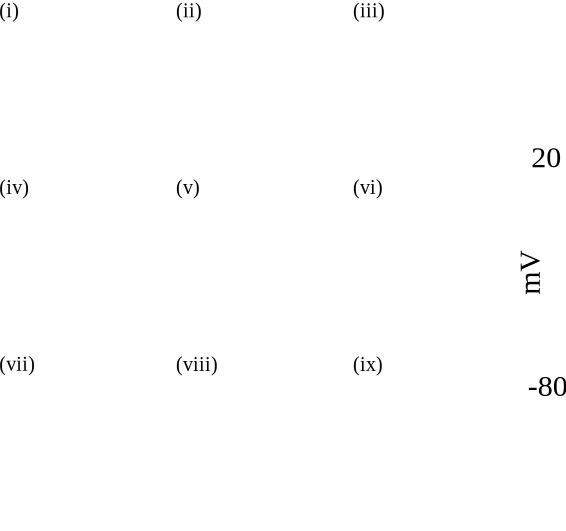
\includegraphics{figures/atrium/validation/front_activation}
\caption[Snapshots of Electrical Activation under Sinus Rhythm (frontal)]{
\label{fig:atrium:validation:main}
Simulated propagation of electrical excitation over the atrial model.
Excitation is initiated in the region corresponding to the sinus node.
Excitation spreads fastest along the fibres of the crista terminalis and the
pectinate muscles.
Snapshots shown for \ms{10}\ (i), \ms{15}\ (ii), \ms{20}\ (iii), \ms{25}\ (iv),
\ms{40}\ (v), \ms{60}\ (vi), \ms{180}\ (vii), \ms{200}\ (viii) and \ms{220}\ (ix).
}
\end{figure}

\begin{figure}
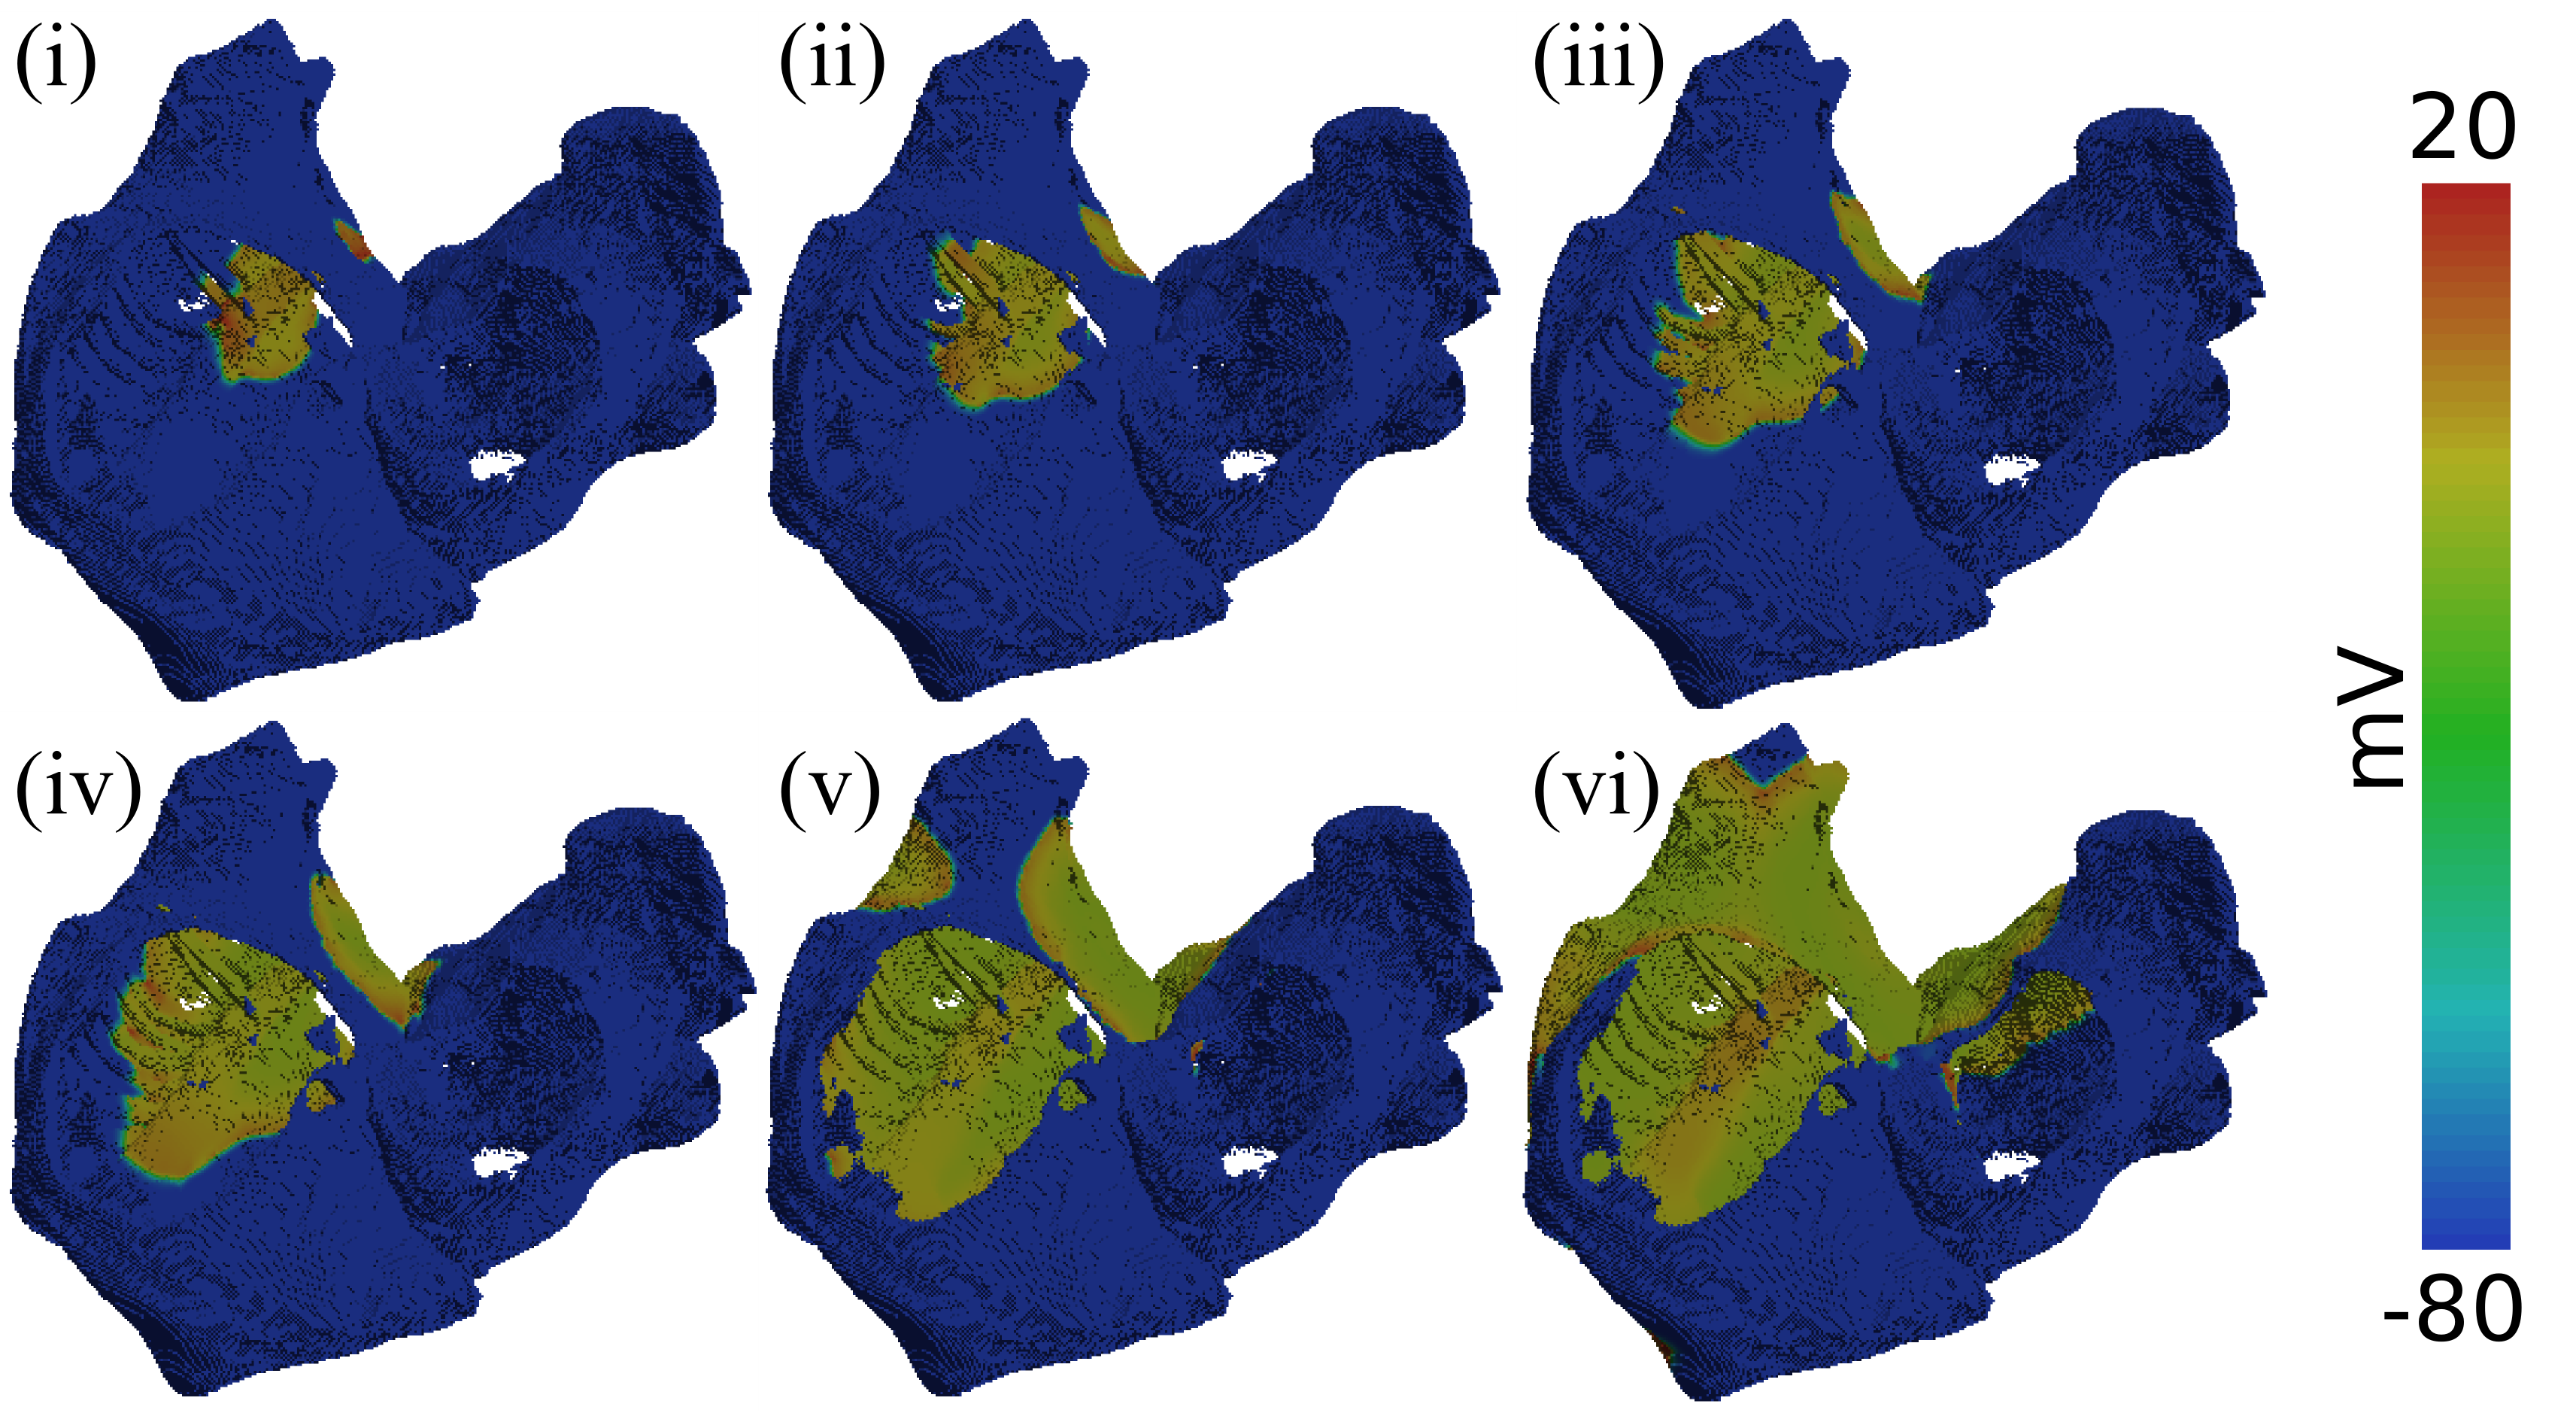
\includegraphics{figures/atrium/validation/back_activation}
\caption[Snapshots of Electrical Activation under Sinus Rhythm (from ventricular
openings)]{
\label{fig:atrium:validation:valves}
Simulated propagation of electrical excitation over the atrial model.
Excitation is initiated in the region corresponding to the sinus node.
Excitation spreads fastest along the fibres of the crista terminalis and the
pectinate muscles.
Snapshots shown for \ms{10}\ (i), \ms{15}\ (ii), \ms{20}\ (iii), \ms{25}\ (iv),
\ms{40}\ (v), \ms{60}\ (vi).
}
\end{figure}

\begin{figure}
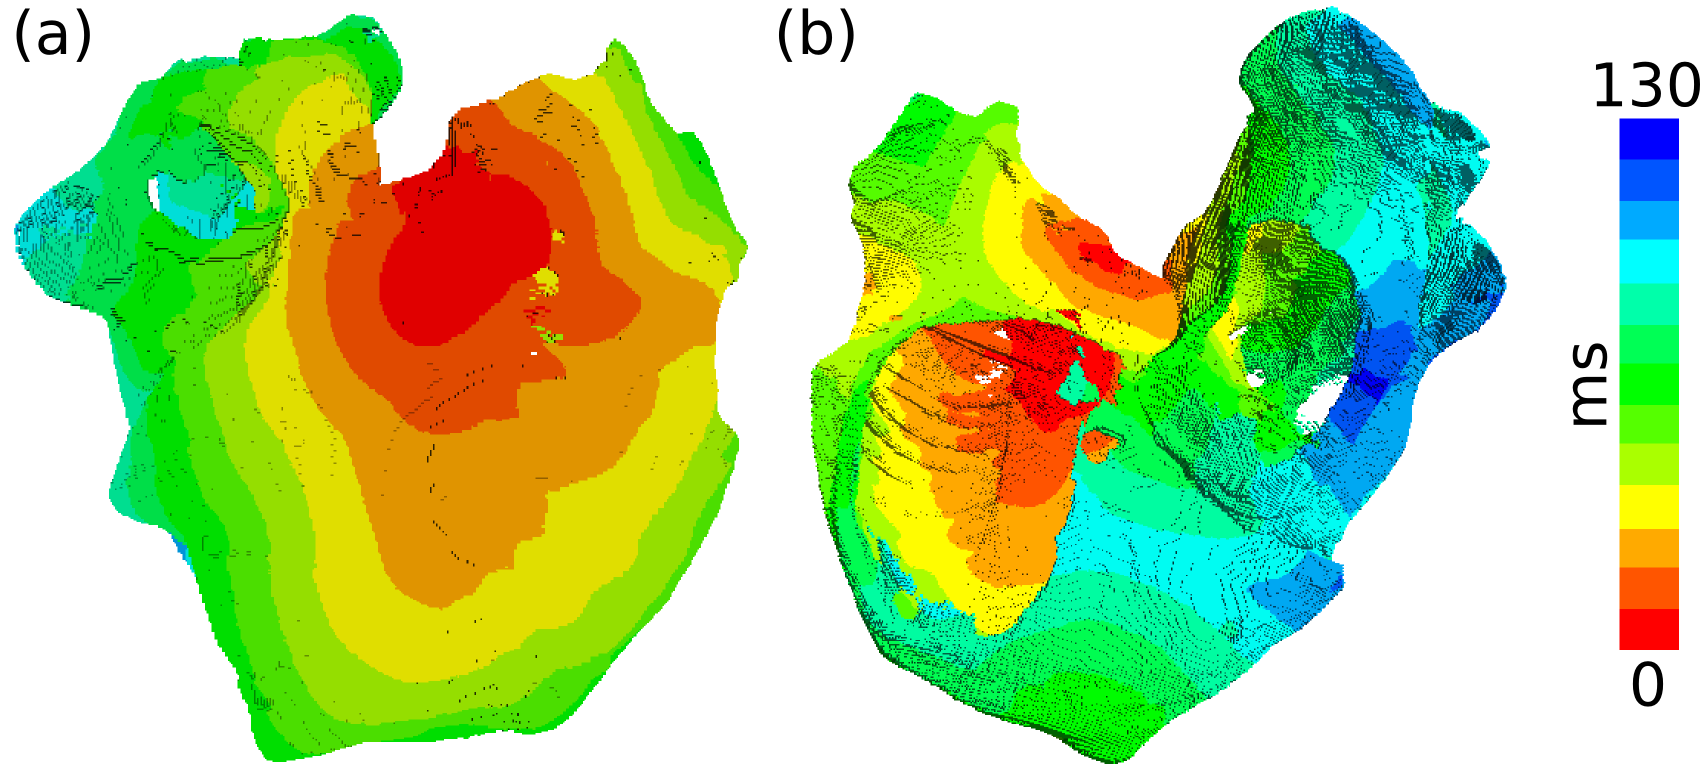
\includegraphics{figures/atrium/validation/activation_times}
\caption[Activation Times Under Sinus Rhythm]{
\label{fig:atrium:validation:times}
Activation times of the atrial geometry from a frontal view (a) and a
view from the ventricles up into the atria (b).
The influence of fibres on the activation times is clearly visible on both
views.
Excitation begins and the sinus node and spreads along the fibres over the
atrial epi- and endocardial surfaces.
The appendages are the last to activate.
}
\end{figure}

Once activated, the whole atrium takes \ms{121}\ to depolarise.
Time to depolarisation was taken as the time for a myocyte to attain a potential
of \mv{-60}.
The site of first activation of the endocardial surface of the left atrium
occurs at \ms{26}\ in the region of the Bachmann's bundle.
The time to total depolarisation of the endocardial surface was \ms{95}\ for
the right atrium and \ms{94}\ for the left atrium.
Conduction velocities were estimated from surface activation time information.
Conduction velocities are found to be $\text{1.30}\pm
0.05\,\text{ms}^{\text{-1}}$ in CT and $\text{0.75}\pm
0.06\,\text{ms}^{\text{-1}}$
in the atrial wall.


\subsection{Comparisons with Experimental Studies}

In a recent patient study Lemery et al. performed simultaneous recordings of
extracellular potentials on the endocardial surfaces of the atria of twenty
patients before they underwent catheter ablation therapy.
They found the total activation time under sinus rhythm for the endocardial
surfaces of both atria was \ms{120}.
The total activation time for the right and left atria was found to be \ms{81}\
and \ms{80}\ respectively.
The time to first activation of the left atrium at the Bachmann's bundle was
found to be \ms{41}.
The results from the simulated propagation are within the range of results
measured clinically for all times and within one SD of the mean for all
quantities except the left atrial activation time.

Conduction velocities for the classes of tissue present in the model have been
measured experimentally as \unit{0.68}{m/s}---\unit{1.03}{m/s}\ for atrial wall
muscle~\cite{Hansson1998}, \unit{0.7}{m/s}---\unit{1.3}{m/s}\ for crista
terminalis~\cite{Boineau1988} in the human atrium.
Conduction velocity in the pectinate muscles or bachmann bundle has not been
measured experimentally in human studies.
The measured conduction velocities are within the experimental limits, providing
further confirmation.

\subsection{Comparisons with Existing Models}

There are several existing three dimensional models of conduction in the whole
human atrium~\cite{Harrild2000,Zemlin2000,Vigmond2001,Seemann2006}\ which use
some variant of a biophysical model for the atria.
Others, such as the cellular automaton approaches~\cite{Reumann2007} are not discussed here.
They represent a range of electrophysiological detail, fibre structure and
computational complexity.
The model of Harrild and Herenriqez~\cite{Harrild2000}\ has a detailed fibre
structure, but this is coupled with homogeneous electrophysiology.
In addition, the model has a relatively coarse space step, with an average
inter-element distance of \mm{0.55}.
The Zemlin~\cite{Zemlin2000}\ model was also based on the visible human dataset.
They used a reduced formulation of the Courtemanche et al. model which has 6
variables.
They included atrial wall muscle fibres based on dissection of anatomical
specimens.
There was no internal fibre structure such as the Bachmann bundle however.
It is a very efficient model.
The Vigmond~\cite{Vigmond2001}\ is an idealised model of an unusual construction.
It is topologically, rather than anatomically, correct and formulated as a
series of shells, made up of interconnected fibres.
The fibre based construction allows for efficient solutions.
The Seemann~\cite{Seemann2006}\ model is closely related to the model proposed in this
chapter--it would be accurate to say that this model is a simplification or
refinement of the Seemann model. 
The Seemann et al. model features an autoactive sino-atrial node complex, while
the model here focuses on the atrial conduction only.
It uses a full formulation of the Courtemanche et al model, without lookup
tables.
It features regions of differing bulk conductivity.
It is much more computationally demanding than the model proposed in this
chapter.

The model of the whole atrium proposed in this chapter represents a compromise
between electrophysiological detail and computational efficiency.
It includes differential electrophysiology and fibre orientation.
The omission of a functioning sino-atrial node is not a large flaw--many
pathological simulations involve non-physiological pacing protocols.
The additional incorporation of an MPI, rather than OpenMP, based implementation
would allow much more distributed execution, allowing long term simulations to
be performed.



\section{Mutation in KCNQ1: A Simulation Study}

Atrial Fibrillation (AF) is the most common arrhythmia in the developed world.
It is a self-promoting condition, with paroxysmal AF episodes frequently
degenerating into chronic and even permanent AF.
Clinically, AF patients show an erratic and high frequency ECG.
At the cellular level, AF is characterised by an abbreviated action potential
(AP) which has no plateau phase and poor heart rate adaptability.
The mechanisms through which AF influences the heart are complex, but the
remodelling of the cellular electrophysiology is believed to contribute to
reduced ERPs and through that, favour the formation of stable, long lived
spiral waves and organ level microwavelet re-entry.
AF is often preceded by congestive heart failure, cardiomegaly and other
structural cardiac diseases, but there are significant numbers of suffers with
no such structural defects.
There is also evidence of a genetic predisposition to AF, which is sometimes
termed Familial Atrial Fibrillation.
Several gene mutations have been causally implicated for AF, leading to AF
which manifests both with and without associated structural cardiac disorders.
The ion channels associated with the repolarization reserve (\ii{K1}, \ii{Kr},
\ii{Ks}) are particularly important to the genesis of AF.
Alterations in functions, gating and kinetics have been implicated in both short
and long QT syndromes.
The \ii{Ks}\ channel has very slow activation kinetics which enable it to
regulate cardiac APs over a wide range of plateau voltages.
Mutations in the \ii{Ks}\ channel are common.
Several mutations in the $\alpha$-subunit, coded for by the KCNQ1 gene, of the
\ii{Ks}\ channel have been identified including both loss-of-function and
gain-of-function, leading to the SQT syndrome and to AF.
Chen et al. studied a four generation Chinese family with hereditary persistent
AF.
They identified a missense mutation at nucleotide 418 from adenine to guanine
resulting in a change from serine to glycine at position 140 (S140G mutation of
\ii{Ks}).
This missense mutation lead to a large gain-of-function which included changes
in the channel kinetics.
It has been hypothesised that these changes in the function of the \ii{Ks}\
channel in the human atrium result in abbreviations of both APD and ERP and thus
provide an appropriate substrate for the genesis of AF.

This study had two goals: To construct a computer model of the available
experimental data from Chen et al. and to then use this model to quantify the
effects of the mutation through the use of cellular, 1D, 2D and 3D models

\subsubsection{Modelling the Mutation}

This study, as in the previous chapter, uses the CRN model, developed by
Courtemanche et al.~\cite{CRN98}\ for simulation of the human atrial action
potential.
As a biophysically detailed model with 21 state variables and numerous ion
channels it is ideal for use in mutation studies.
The CRN model has individual descriptions of several $K^{+}$\ currents.
These include the time-independent potassium current, \ii{K1}, the ultra-rapid
potassium current, \ii{Kur}, the transient outward current, \ii{to}\ and the
rapid and slow delayed rectifier currents, \ii{Kr}\ and \ii{Ks}.
The latter current is modulated by the mutation and is described in the control
CRN cell by
\begin{equation}
\label{atrium:iks_con}
\ii{Ks} = g_{Ks}x_{s}^{2}\left(V-E_{K}\right)
\end{equation}
where $g_{\tiny{Ks}}$\ is the channel conductance (\unit{0.129}{nS/pF}), $x_{s}$\ is
the activation variable and $E_{K}$\ is the $K^{+}$\ reversal potential, found
through the Nernst potential.

\subsubsection{Simulation of the S140G mutation of KCNQ1 I-V relationship}

The Chen et al.~\cite{Chen2003} study determined that the most likely cause of
familial AF was was the S140G mutation of the KCQN1 gene, which forms part of
the $\alpha$-subunit of the \ii{Ks}\ channel.
The gene was transfected into COS7 cells along with the second component of
the $\alpha$-subunit, KCNE1, in both normal (WT) and mutated type (MT).
The transfected cells were used to perform voltage clamp experiments.
The clamp protocol used is shown in figure~\ref{atrium:iks:vc},A.
This is the experimental protocol used by Chen et al.~\cite{Chen2003}.
The cell was held at a holding potential of \mv{80} for \unit{0.5}{s}\ before
being held at \mv{10}\ steps between \mv{-130}\ to \mv{50}\ for \unit{3}{s}.
The voltage steps were followed by a \mv{-40}\ holding potential, applied for
\unit{1}{s}.
The values of \ii{Ks} at the end of the step voltages were plotted against the
step voltages to determine  I-V relationships for WT
and MT cells, shown in figure~\ref{atrium:iks:vc},B (points with errors) and
current traces, shown in figure~\ref{atrium:iks:vc},C and D for WT and MT,
respectively.

\begin{figure}
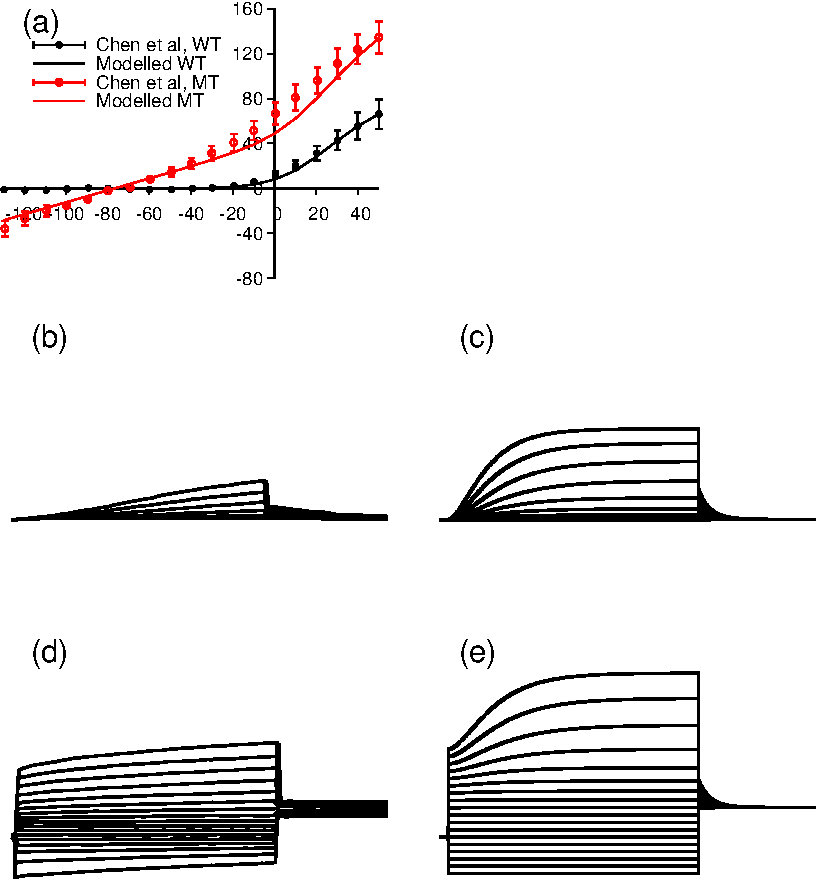
\includegraphics{figures/atrium/iks/figures/01_IV}
\caption[KCNQ1 mutation in IKs, experimental data]{
\label{atrium:iks:vc}
(a) Voltage clamp protocol used by Chen et al.~\cite{Chen2003}.
(b) Experimental WT (black, closed circles) and MT (red, open circles)
I-V relationships recorded by Chen et al.  Simulated I-V curves for WT (black
lines) and MT (red lines).  Modelled curves are scaled to experimental points
based on the WT current density at \mv{50}.
(c) Experimental current traces for WT.
(d) Simulated current traces for WT.
(e) Experimental current traces for MT.  Note the instantaneous
activation, and the significant inward current at negative clamp potentials.
(f) Simulated current traces for MT.
}
\end{figure}

The I-V relationship shows that the mutation causes a gain-of-function across
all the clamp potentials.
It also reveals that the mutation appears to cause an inward current at negative
potentials.
The current traces suggest a drastic change in the kinetics of the \ii{Ks}\
channel with a significant component of the current being activated immediately.
The addition of a leakage component to (\ref{atrium:iks_con}) allowed simulation
of \ii{Ks}\ characteristics which closely matched the experimental data.
Under MT conditions, the new total current \iip{Ks}\ was described by
\begin{equation}
\label{atrium:iks_mut}
\iip{Ks} = \ii{Ks} + \varphi g_{Ks}x\left(V-E_{rev}\right)
\end{equation}
where \ii{Ks}\ is (\ref{atrium:iks_con}), $\varphi$\ is a multiplicative parameter
from with values between 0 and 1, $g_{Ks}$ is as in (\ref{atrium:iks_con}) and
$E_{rev}$\ is the reversal potential of the leakage component.
The reversal potential was estimated from the experimental I-V relationships to be
\mv{-76.3}.
The inclusion of the $\varphi$\ parameter allowed the simulation of several
intermediate mutant states, representative of a heterozygous mutation.
Setting $\varphi = 1$\ and following the voltage clamp protocol shown in panel A
of figure~\ref{atrium:iks:vc}\ the I-V relationship of \ii{Ks}\ was simulated to
provide a good match to experimental data shown as the lines in panel B of
figure~\ref{atrium:iks:vc}.
Also shown are the simulated current traces elicited by the voltage clamp
protocol in panels D and F.
The non-gated leakage component of \iip{Ks}\ sufficiently accounts for the
changed current density and kinetics.

\subsubsection{Simulation Protocols}
\label{sec:atrium:s140g:methods}
To assess the effects of the mutation on human atrial myocytes, cellular models
including the modified \iip{Ks}\ described by (\ref{atrium:iks_mut}) were used
in a number of simulation protocols, as described in Chapter 2.
Initially the \apd\ was evaluated under conditions corresponding to $\varphi =
0$\ (WT) and $\varphi = 1$\ (MT).
Under such conditions, the induced \apd\ shortening was found to result in
un-physiological \apd\ values, shown in figure \ref{atrium:iks:apd}.
Therefore a pair of heterozygous cases, corresponding to $\varphi = 0.10$\
(HT10) and $\varphi = 0.25$\ (HT25) were created and used in the evaluation of
the mutation's effects.

Using the models and protocols described in Chapter 2 the \apdr, ERP\emph{r}, VW,
CV\emph{r}, SVW and the dynamic behaviours of spiral waves were evaluated for
the WT, HT10 and HT25 cases.
For the 3D simulations, the model described in Sections
\ref{atrium:sec:geometry}\ and \ref{atrium:sec:model}\ was used.
Since the intention was just to investigate the influence of the mutation, the
model was used without tissue anisotropy.
The mutation was applied homogeneously with the electrical activity at all
nodes described by either the WT or HT25 cells.
There was no heterogeneity introduced to account for the differing cell types
present in the human atrium.
To examine the behaviour of scroll waves under WT and HT25 conditions a protocol
analogous to the wave-break protocol described for 2D sheets of tissue was
used~\cite{Kharche2007}.
The protocol is illustrated in figure~\ref{atrium:iks:scroll_init}.
\begin{figure}
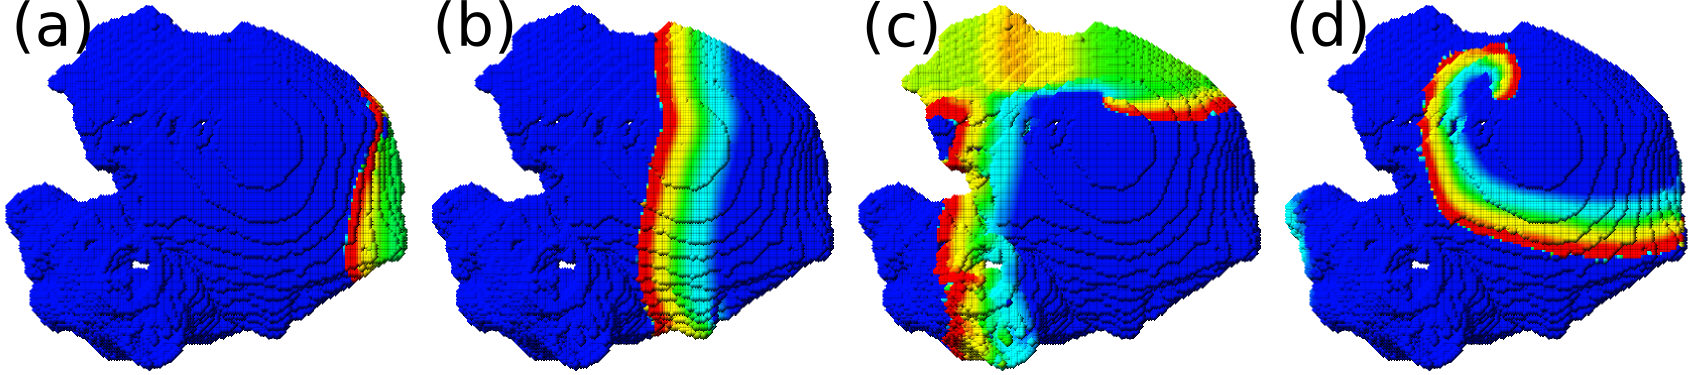
\includegraphics{figures/atrium/iks/scrollhowto}
\caption[Initiating a Scroll Wave]{
\label{atrium:iks:scroll_init}
Stimulus protocol used to initiate a scroll wave.
(a) One extreme of the atrial model is stimulated
(b) The excitation is allowed to propagate
(c) An S2 stimulus is delivered by clamping a section of the tissue, here
the lower quarter.
(d) A scroll wave begins on the wall of the right atrium.
}
\end{figure}
First, a small number of cells are simulated at one extreme of the atrial model.
The excitation is allowed to propagate through the model until the S2 stimulus
is delivered.
The S2 stimulus is delivered via briefly clamping a section of the atrial model to
\mv{50}\ and then releasing the clamp.
A correctly timed S2 stimulus results in a scroll wave on the wall of the right
atrium.
After initiation, the models were simulated until activity ceased or until
\unit{6}{s}\ of simulated time had elapsed.

\subsubsection{Changes in \apd\ due to S140G mutation}

The effect of an increase in the leakage current parameter were investigated.
This was done using the standard \apd\ protocol and varying $\varphi$\ between
0 and 1.
Variation in \apd\ as $\varphi$\ is altered is shown in
figure~\ref{atrium:iks:apd}(a).
Representative APs are shown in figure~\ref{atrium:iks:apd}(b).
The \apd\ under Control conditions (WT) was seen to be \ms{312.0}.
Progressive mutation decreased the \apd\ to \ms{150.5}\ in HT10 case and
\ms{79.3}\ in HT25 case.
Under homozygous conditions, $\varphi = 1$\, the \apd\ was seen to be \ms{22.4}.
Figure~\ref{atrium:iks:apd}(b) shows the inclusion of the mutant channel causes
the changes in morphology associated with none of the mutant types having a
plateau region.
Inclusion of the mutant channel decreased the upstroke velocity of the AP from
\unit{217.1}{V/s}\ in WT, to \unit{214.0}{V/s}\ in HT10 and \unit{208.6}{V/s}\
in HT25.
The upstroke velocity in the homozygous case was \unit{192.0}{V/s}.
\begin{figure}
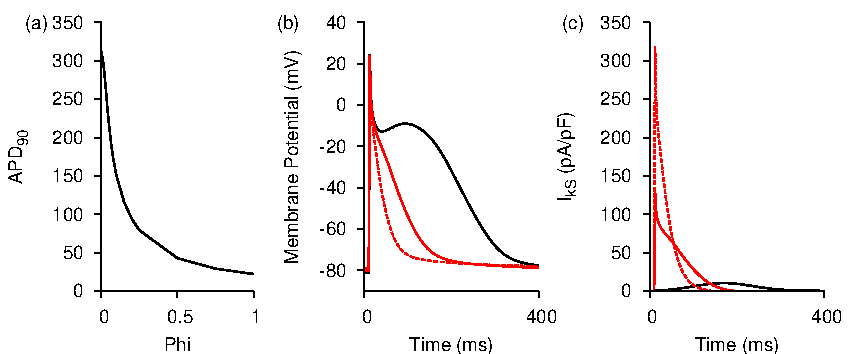
\includegraphics{figures/atrium/iks/figures/02_APD}
\caption[AP and current profiles with S140G mutation]{
\label{atrium:iks:apd}
(a) Plot of \apd\ vs $\varphi$, showing how increasing mutation reduces \apd.
AP profiles (a) and \ii{Ks}\ current profiles (b) for WT (black), HT10 (red,
solid) and HT25 (red, dashed).
Stimulus is delivered at \ms{10}.
Note the large increase in current density under the S140G mutation, which
causes a corresponding flattening of the AP profiles and removal of the plateau.
}
\end{figure}
Figure~\ref{atrium:iks:apd}(c) shows the current profiles of \ii{Ks} over the course of
an AP which correspond to the AP traces shown in panel B.
\ii{Ks}\ is seen to increase considerably in both the HT10 and HT25 cases
compared with the WT case.
The leak also changes the morphology of the current profile to one showing
almost instant activation in HT10 and HT25 cases, compared to the slow
activation in WT.

\subsubsection{\apdr\, ERP\emph{r}, CV\emph{r} and VW}

\begin{figure}
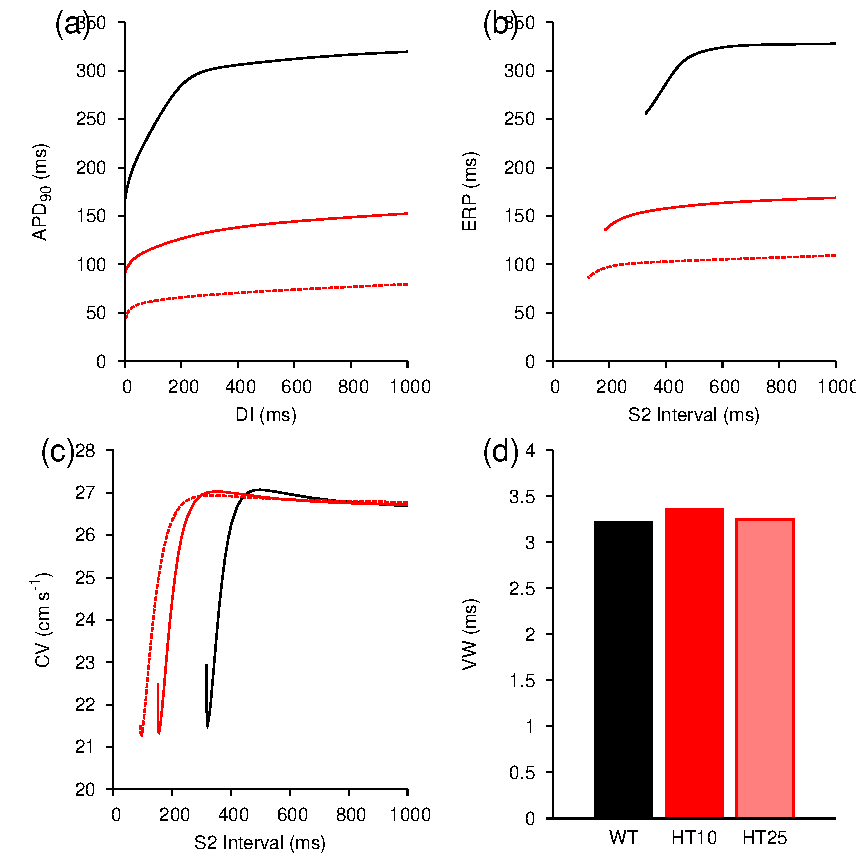
\includegraphics{figures/atrium/iks/figures/03_REST}
\caption[Restitution properties with S140G mutation]{
\label{atrium:iks:apdretal}
Restitution curves for WT (black), HT10 (red, solid) and HT25 (red, dashed).
(a) \apdr.
(b) ERP\emph{r}.
(c) CV\emph{r}.
(d) Temporal VW to premature stimulus.
}
\end{figure}

The \apdr\, figure~\ref{atrium:iks:apdretal}(a), reflects the decreased \apd\ with
the restitution curves considerably flattened for both the mutant cases.
The ERP\emph{r}\ curves, figure~\ref{atrium:iks:apdretal}(b), also reflect the
reduced \apd\ and show a similar flattening to that seen in the \apdr\ curves.
At an S1 interval of \ms{1000}\ the ERP was found to be \ms{327.2}\ in WT,
\ms{168.4} in HT10 and \ms{109.3} in HT25.
In addition, the mutant cases supported excitation at much lower S1 intervals
(or higher pacing rate) compared to the control case.
The minimum S1 interval sustained during the ERP\emph{r}\ calculations was
\ms{328.7}\ in WT, \ms{184.3} in HT10 and \ms{126.7} in HT25.
The solitary wave CV was not altered considerably by the mutation (\cms{26.7}\
in WT c.f. \cms{26.8} in HT25).
The CV\emph{r}\, figure~\ref{atrium:iks:apdretal}(c), curves confirm the findings
of the ERP\emph{r}\ calculations, that the mutant case supports successful
excitation after a considerably reduced S2 interval.
The minimum S2 interval which still allowed the test stimulus to propagate was
found to be \ms{317.1}\ in WT, \ms{151.7}\ in HT10 and \ms{92.5}\ in HT25.
Vulnerability to premature excitation was relatively unaffected by the mutation.
It was observed to increase in tissues where the mutation was present from a VW of
\ms{3.2}\ in WT to \ms{3.4}\ in HT10 and \ms{3.3}\ in HT25
(figure~\ref{atrium:iks:apdretal}(d)).
This is a small (less than 5~\%) change in the VW to premature excitation.

\subsubsection{Dynamic Behaviours on a 2D sheet}

Re-entry was initiated in 2D sheets of homogeneous virtual human atrial tissues
for WT, HT10 and HT25 cases.
The dynamical behaviours of the system were observed for \unit{10}{s}\ or until
all electrical activity ceased after the re-entry self terminated.
Frames from the simulation and spiral tip traces are shown in
figure~\ref{atrium:iks:twodframes}.
The lifespan of re-entrant waves in the WT case was seen to be \unit{2.8}{s},
whilst in both the HT10 and HT25 cases the re-entry persisted for the duration
of the simulation (\unit{10}{s}).
In the WT case the spiral tip showed a large degree of meander
(figure~\ref{atrium:iks:twodframes},top row, column iv) even after the initial
transitory period.
The tip trajectory shows that the spiral wave completes several rotations, each
accompanied by large movements of the tip before finally tip exits along the
lower edge of the tissue, unable to move back into the tissue due to its own
refractory tail.
In contrast in both HT10 and HT25 cases the meander is confined to a relatively
small area after after the initial transitory period.
The spiral wave tip precesses around a stationary point in a flower petal
pattern, indicative of a highly stable re-entrant wave.

\begin{figure}
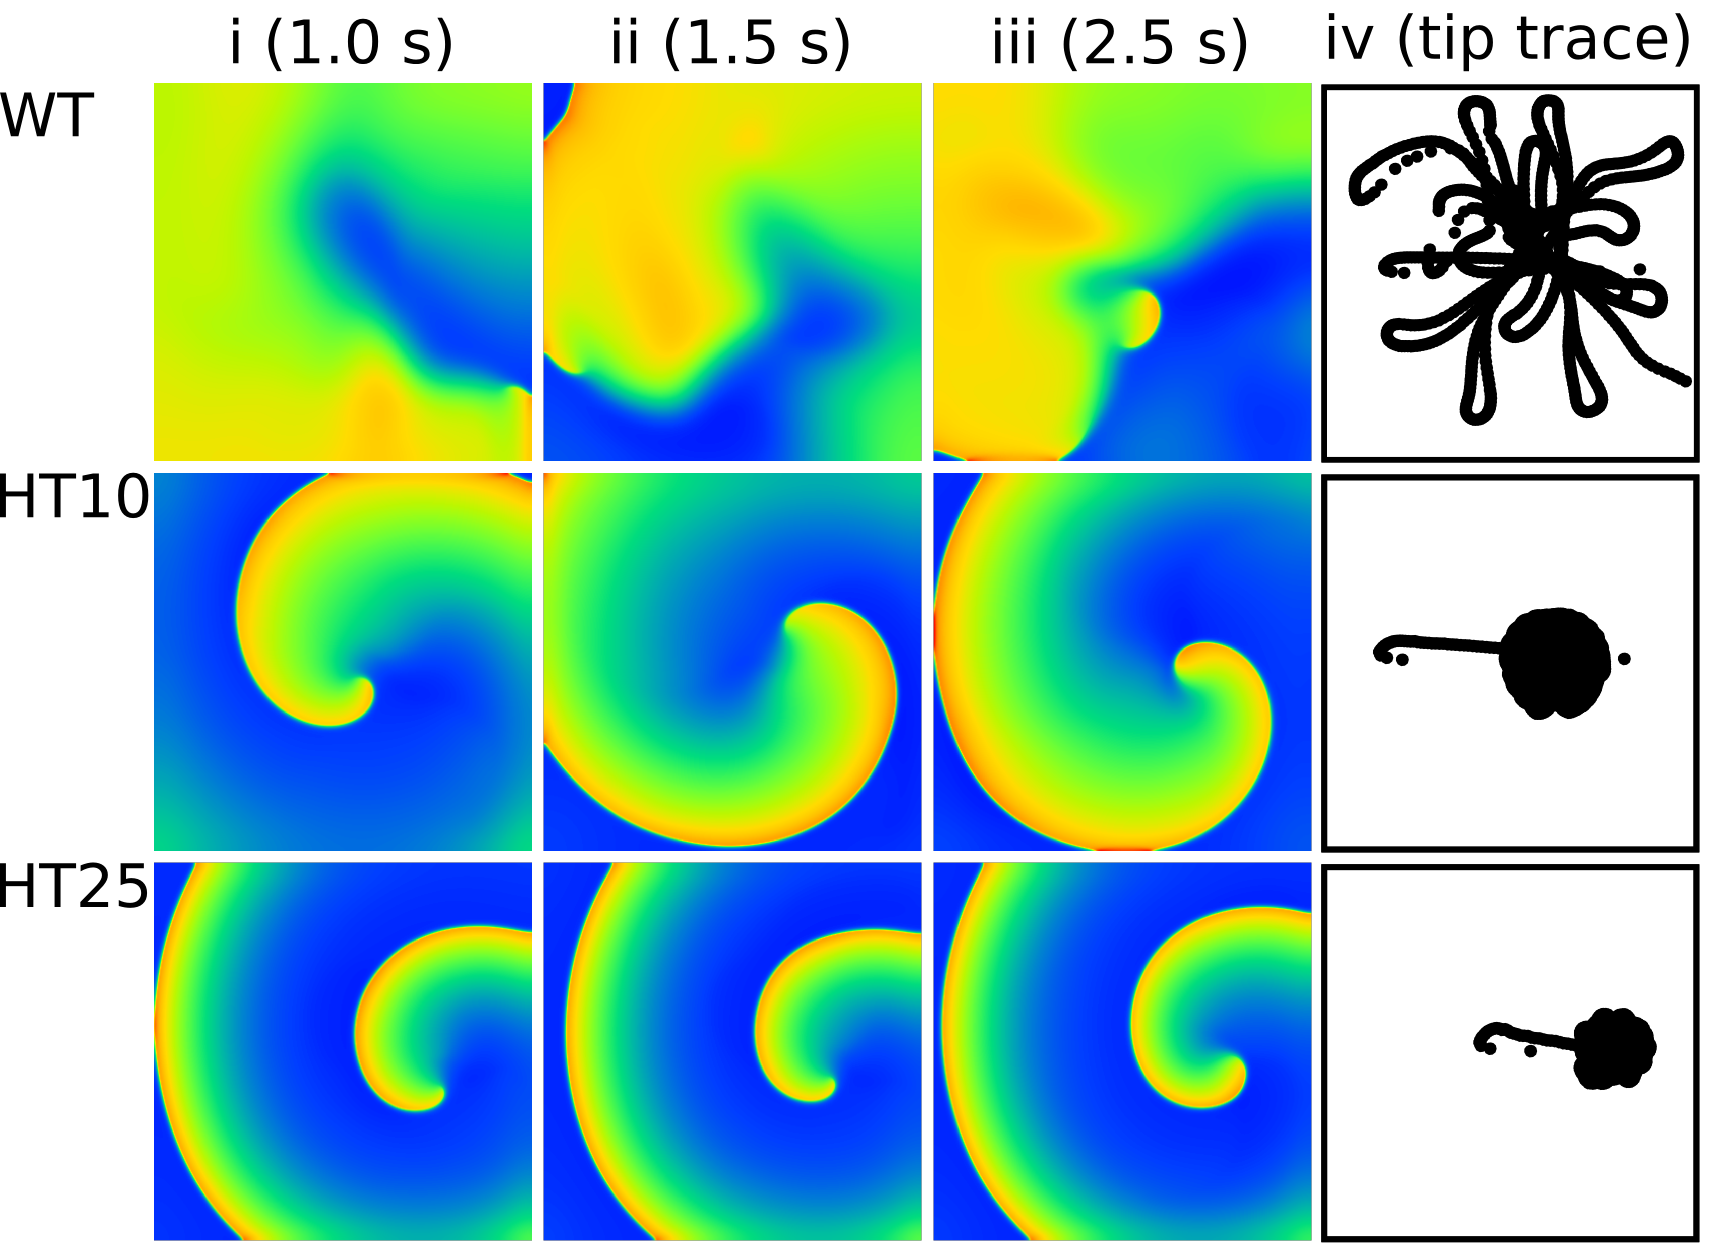
\includegraphics{figures/atrium/iks/2Dplots}
\caption[2D Re-entry under S140G conditions]{
\label{atrium:iks:twodframes}
Snapshots of electrical activity extracted at \unit{1}{s}\ (i), \unit{1.5}{s}\
(ii) and \unit{2.5}{s}\ (iii) after spiral wave initiation, with accompanying
tip trace shown in (IV) for WT (top), HT10 (middle) and HT25 (bottom).  In the
electrical activity plots red is fully depolarized, blue is the resting
potential.  The WT spiral occupies much more of the tissue and has a very large
meander, compared with the HT10 and HT25 cases, which show a very stable spiral
after the initial transient behaviour.
}
\end{figure}

Representative APs were extracted from a point in the tissue and used in
dominant frequency analysis, shown in figure~\ref{atrium:iks:twodfreq}.
From the representative APs (top panels) it can be seen that the \apd\ decreases
as a greater proportion of the mutation is present.
The WT case also shows obvious alternans in the AP profiles reflecting its
unstable and meandering spiral wave, contrasting with the general uniform APs
seen with the HT10 and HT25 cases.
Dominant frequency analysis of AP profiles (bottom panels) extracted along the
sheet diagonal was performed.
The dominant frequency analysis shows that whilst in the WT case there is a
relatively low frequency of oscillations (less than \unit{4}{Hz}) compared with
the mutant cases (\unit{7}{Hz} in HT10, \unit{10}{Hz} in HT25).
The width of the peaks for the two mutant cases are smaller, indicating a
greater stability compared to the more dispersed frequencies seen in the WT
case.

\begin{figure}
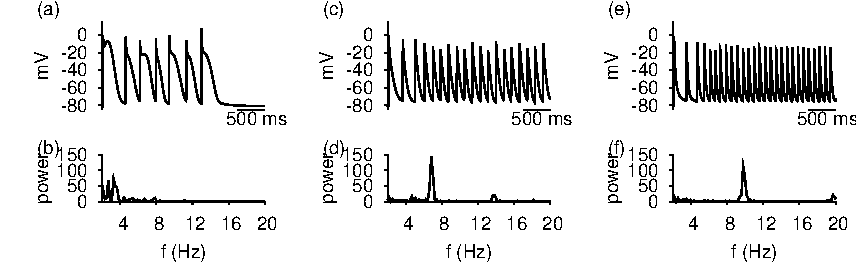
\includegraphics{figures/atrium/iks/figures/05_2D_freq}
\caption[Frequency of extracted APs from 2D sheets with S140G mutation]{
\label{atrium:iks:twodfreq}
Representative AP traces (top panels) and dominant frequency analysis (bottom
panels) for WT (left), HT10 (centre) and HT25 (right).  Traces extracted from a
point \mm{6}\ from top and left of the 2D sheets every \ms{2.5} of elapsed time.
}
\end{figure}

The minimal stimulus substrate size was computed as shown in
figure~\ref{atrium:iks:svw}.
The mutation induced remodelling dramatically reduced the size of the SVW, from
\mm{99.1}\ in WT conditions to \mm{12.3}\ in HT25 conditions, a reduction of
87.5\%.

\begin{figure}
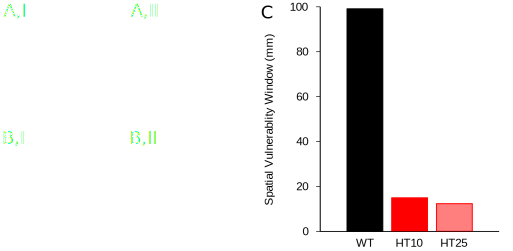
\includegraphics{figures/atrium/iks/07_svw}
\caption[Spatial Vulnerability Window with S140G mutation]{
\label{atrium:iks:svw}
(a) Unsuccessful attempt at initiating figure-of-eight re-entry just
before (I) and after (II) re-entry would occur.
(b) Successful initiation of figure-of-eight re-entry just before (I) and
just after (II) re-entry is initiated.
(c) Spatial vulnerability window for WT (black), HT10 (red) and HT25
(pink) tissue.
Spatial vulnerability window is the minimum length of tissue that produces
figure-of-eight re-entry.
}
\end{figure}

\subsubsection{Modelling the S140G mutation in the Whole Atrium}

Scroll waves were initiated in the whole atrial model as described in
\ref{sec:atrium:s140g:methods}.
Scroll wave behaviour for control (WT) and $\varphi = 0.25$\ (HT25) were studied
as representative cases.
The scroll waves were initiated on the right atrial free wall to allow
initiation and initial evolution without interference with anatomical obstacles.
The 3D simulation visualisations are presented in
figure~\ref{atrium:iks:threed}.
In WT conditions, as observed in the 2D simulations, the scroll waves have a
large meander and self-terminated in approximately \unit{4.2}{s}.
As long as the scroll wave was initiated far from anatomical obstacles such as
venous openings, self-termination was independent of position.
In certain cases where it was not `entrapment' of the scroll wave around an
anatomical obstacle was observed, leading to prolonged scroll wave activity even
in the WT case.
Under HT25 conditions the small wavelength allowed scroll waves to become
persistent in all cases, as observed in 2D simulations.
In contrast to the 2D simulations the presence of anatomical obstacles led to break up of the
scroll wave into erratic propagations and short-lived wavelets.
This erratic behaviour then persisted until the end of simulation at
\unit{6}{s}.

\begin{figure}
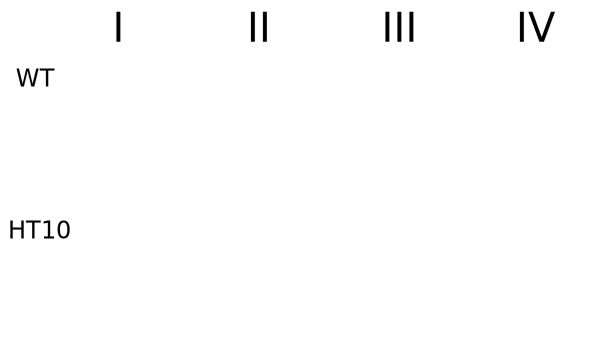
\includegraphics{figures/atrium/iks/3D_Fig}
\caption[Snapshots of membrane potential over the whole atrium with S140G
mutation]{
\label{atrium:iks:threed}
Snapshots of the membrane potential for WT (top panels) and HT25 (bottom
panels) taken at \unit{1}{s} (i), \unit{2}{s} (ii), \unit{3}{s} (iii) and
\unit{4}{s} (iv) of simulated time.
In the plots, red shows full depolarized tissue, whilst blue tissue is at rest.
By \unit{2}{s} the activity shown in panel bottom,ii has started to break up, compared with
the more stable ave shown in the upper panel, just about to self-terminate in
panel top,iv, as the excitation wavefront hits the non-conducting atrio-ventricular
ring.
}
\end{figure}

Representative AP profiles were extracted from several points throughout the
atrial model and used in dominant frequency analysis.
The dominant frequency in the HT25 case was found to be much higher,
approximately \unit{10}{Hz}, than in the WT case, less than \unit{3}{Hz}.
%This is shown in figure~\ref{atrium:iks:threeddf}.

\subsubsection{Discussion and Conclusions of the S140G Study}

The S140G mutation of the KCNQ1 $\beta$\ subunit of the \ii{Ks}\ ion channel
causes a large gain of function.
This gain of function manifests as a component of the \ii{Ks}\ channel which
shows instantaneous activation kinetics under voltage clamp conditions.
Modelling the effects of the mutation as the addition of a leakage component
with constant conductance to the \ii{Ks}\ channel therefore seems to be a good
fit to the experimental data provided by Chen et al.
Incorporation of the mutation into models of cellular electrophysiology
dramatically reduces the \apd\ and the ERP.
The increased repolarization current also flattens the plateau region, or
eliminates it entirely.
Conduction velocity was not significantly affected by the presence of the
mutation, possibly due to the leakage component being inward at resting
potentials, contributing to the upstroke.
In 2D simulations, the mutation stabilised re-entrant spiral waves, leading to
long lived arrhythmic activity at a high frequency.
In 3D, simulations showed that with the addition of anatomical obstacles,
scroll-waves would instead break up.
The shorter wavelength and refractory length introduced by the mutation assists
in the maintenance of the fibrillatory activity.
The fibrillatory activity in the presence of the mutation shows a very high
frequency, approximately \unit{600}{bpm}, which is in agreement with the
definition Chen et al. used when selecting AF sufferers for their study.
The Chen et al. hypothesis is supported by this study, which reproduces both
voltage clamp experiments and then provides insight into the mechanisms
responsible for the maintenance of AF in those afflicted with the mutation.

Repolarisation of cardiac myocytes depends on the \ii{Ks}\ (KCNQ1/KCNE1) and
\ii{Kr}\ (hERG) channels.
Previous clinical and simulation studies have linked mutation leading to
gain of function in the \ii{Ks}\ to SQT syndromes~\cite{Brugada2004,Hong2005}.
Studies by Bosch and Workmann into AF induced remodelling focused on the
\ii{K1}\ and \ii{to}\ potassium channels, as well as the L-type calcium channel.
Atrial \ii{Ks}\ is a much lower magnitude than ventricular \ii{Ks}\ so its
upregulation may have been overlooked in their studies.
The simulations shows that \ii{Ks}\ has an important role to play in the behaviour
of atrial cell electrophysiology and that gain of function mutations in the
channel can lead to a large reduction in the \apd\ and ERP.

This study was carried out using a model of the human atria which omitted
spatial and electrical heterogeneity.
This allowed the mutation to be studied without the additional complexity
introduced by heterogeneity.
In addition, it is well known that AF can induce significant structural
remodelling~\cite{Goette2002,Avitall2008} with most AF observed in clinical settings accompanied by cardiac
structural disorders.
Inter-myocyte coupling can also be influenced~\cite{Velden1998}\ by chronic
atrial fibrillation.
Such etiology is beyond the scope of this study and would be a significant
investigation in its own right.
Despite the relative simplicity of the study in 3D, the control cases still show
self-termination as expected, whilst the presence of the mutation leads to
breakup and fibrillation.
Simulation studies allow modelling of only the aspects of the disease which
interest the investigator.

Electrical remodelling involves complex regulatory mechanisms.
AF is known to be associated with the remodelling of several ion channels.
Recent clinical studies have identified numerous
genes~\cite{Otway2007,Xia2005,Yang2004,Restier2008,Hong2005,Ravens2008,Yang1997a,Olson2005a} responsible for a
propensity towards AF due to reductions in the ERP and \apd.
A recent modelling study of mutation in the KCNJ2 Kir2.1 gene~\cite{Kharche2008}, leading to gain
of function in the \ii{K1}\ channel, was found to lead to dramatic reduction in
ERP and \apd.
An extension of the simulation study into three dimensions showed that it led to
persistent and erratic propagations.
A gain of function in the potassium repolarization currents seems to lead to
behaviour which is qualitatively, if not quantitatively, similar to the study
presented in this chapter.

Computational studies of AF have investigated the effects of AF at both cellular
and tissue levels.
Cellular effects of AF are important and have been explored in several
investigations~\cite{Zhang2005,Workman2001,Bosch2003}.
On the tissue level, Pandit et al. have studied the effects of channel blocking
on 2D propagations\cite{Pandit2005}.
Three dimensional studies have included Reumann et al. who used a cellular
automaton based model of the human atria to study AF~\cite{Reumann2007}.
Such a model, by its nature, does not consider the continuous time variation of
potentials within the human atria, and may accumulate significant error in a
short period of time.

\section{Modelling the Whole Atrium: Conclusion}

A realistic model of the human atria has been developed.
The model uses a biophysically detailed second generation cellular
electrophysiological model to describe the action potential kinetics at each node.
The model includes a simplistic but effective electrophysiological
heterogeneity, in the absence of more detailed experimental data.
Solution times for the model are improved by the use of lookup tables for
voltage dependent values.
The geometry is based on data from a real human dataset.
A simple description of fibre orientation has been included and conduction
anisotropy has been considered.
The resulting whole atrium model has a good parallel fraction and is solvable in
tractable times on modern hardware.

The model accurately reproduces the activation sequence of the healthy human
atrium.
Time to total activation and individual tissue conduction velocities both fall
within experimental values.
Thanks to the use of a biophysically detailed model of cellular action
potential, the model can also be used to simulate pathological cases such as
familial atrial fibrillation.


